\documentclass{article}
\usepackage[utf8]{inputenc}
\usepackage{amsmath}
\usepackage{tabto}
\usepackage{pgfplots}
\usepackage{hyperref}
\usepackage{tikz}
\usepackage{tikz-3dplot}
\title{Rotations and Transformations in 3D}
\author{Intro to Robotics}
\date{}

\begin{document}

\maketitle
\section{Euler Rotation Theorem}
The orientation of one coordinate frame with respect to another can be described by "successive  rotations about the three axes, such that no two successive rotations are about the same axis." \\\\
12 possible rotations: xyz, xzy, yxz, yzx, zxy, zyx; (three different axes) xyx, yxy, xzx, zxz, yzy, zyz(two different axes) \\\\
Given these twelve rotation , you can apply them differently. The two methods of application are fixed angle rotation and eulerian rotation.\\\\
fixed angle rotation(applied backwards):  ${}^{A}_{B}R_{xyz}(\alpha,\beta,\gamma)={}^{A}_{B}R_z(\gamma){}^{A}_{B}R_y(\beta){}^{A}_{B}R_x(\alpha)$\\
Eulerian angle rotation(applied in order): ${}^{A}_{B}R_{x'y'z'}(\alpha,\beta,\gamma)={}^{A}_{B}R_{x'}(\alpha){}^{A}_{B}R_{y'}(\beta){}^{A}_{B}R_{z'}(\gamma)$\\\\

In general we will use the eulerain angle method(x'y'z' the prime indicates eulerian method); combined with  yaw(z), pitch(y), roll(x) parameterization of the angles. Algebraically: ${}^{A}_{B}R_{z'y'x'}(\alpha,\beta,\gamma)$.\\\\
\newpage
\section{Using rotation matrices in 3D}
As previously mentioned, we will be using rotations in eulerian angle form with yaw(z axis), pitch(y axis), and roll(x axis) parameterization. All the 2D rotation matrix properties still hold, A 3D rotation matrix is orthonormal, det(R)=$\pm1$, $R(-\theta)=R^T(\theta)=R^{-1}(\theta)$. Now let us cover the three rotation matrices used for yaw, pitch, and roll.\\
\begin{figure}[htp]
    \centering
    \includegraphics[width=5cm ]{ypr.png}
    \caption{}
    \label{fig:pubsub}
\end{figure}\\\\
Yaw uses the rotation matrix $R_z(\alpha)$, and this is equal to:\\
$R_z(\alpha)=\begin{bmatrix}
c\alpha & -s\alpha & 0 \\
s\alpha & c\alpha & 0\\
0 & 0 & 1
\end{bmatrix}$\\
This rotation matrix allows us to rotate the xy plane by keeping the z axis fixed.\\\\
pitch uses the rotation matrix $R_y(\beta)$, and this is equal to:\\
$R_y(\beta)=\begin{bmatrix}
c\beta & 0 & s\beta \\
0 & 1 & 0\\
-s\beta & 0 & c\beta
\end{bmatrix}$\\
This rotation matrix allows us to rotate the xz plane by keeping the y axis fixed.\\\\
roll uses the rotation matrix $R_x(\gamma)$, and this is equal to:\\
$R_x(\alpha)=\begin{bmatrix}
1 & 0 & 0 \\
0 & c\gamma & -s\gamma\\
0 & s\gamma & c\gamma
\end{bmatrix}$\\
This rotation matrix allows us to rotate the yz plane by keeping the x axis fixed.\\\\
\textbf{More on 3D rotations}\\
Lets say the orientation of an object is $60^\circ$ on the yz plane(x fixed-roll), $17^\circ$ on the xz plane(y fixed-pitch), and $30^\circ$ on the xy plane(z fixed-yaw). I can represent this orientation using eulerian roll-pitch-yaw parameterization $R_{z'y'x'}(\alpha,\beta,\gamma)$.\\\\
$R_{z'y'x'}(\alpha,\beta,\gamma)=R_{z'y'x'}(60^\circ,17^\circ,30^\circ)=R_z(60^\circ)R_y(17^\circ)R_x(30^\circ)=\\ \begin{bmatrix}
c60^\circ & -s60^\circ & 0 \\
s60^\circ & c60^\circ & 0\\
0 & 0 & 1
\end{bmatrix}_{z}\begin{bmatrix}
c17^\circ & 0 & s17^\circ \\
0 & 1 & 0\\
-s17^\circ & 0 & c17^\circ
\end{bmatrix}_{y}\begin{bmatrix}
1 & 0 & 0 \\
0 & c30^\circ & -s30^\circ\\
0 & s30^\circ & c30^\circ
\end{bmatrix}_{x}=\\
\begin{bmatrix}
.5 & -.87 & 0 \\
.87 & .5 & 0\\
0 & 0 & 1
\end{bmatrix}_{z}\begin{bmatrix}
.96 & 0 & .29 \\
0 & 1 & 0\\
-.29 & 0 & .96
\end{bmatrix}_{y}\begin{bmatrix}
1 & 0 & 0 \\
0 & .87 & -.5\\
0 & .5 & .87
\end{bmatrix}_{x}= \\
\begin{bmatrix}
.48 & -.83 & .29\\
.82 & .31 & -.48\\
.31 & .47 & .83
\end{bmatrix}_{z'y'x'}$ \\\\
The easiest way to understand a rotation matrix $R_{z'y'x'}$ is by plotting the column vectors as $R_{z'y'x'}=\begin{bmatrix}
x_{object} & y_{object} & z_{object}    
\end{bmatrix}$ as shown below ($R_{z'y'x'}$ describes how to go from the green frame to the red frame):\\

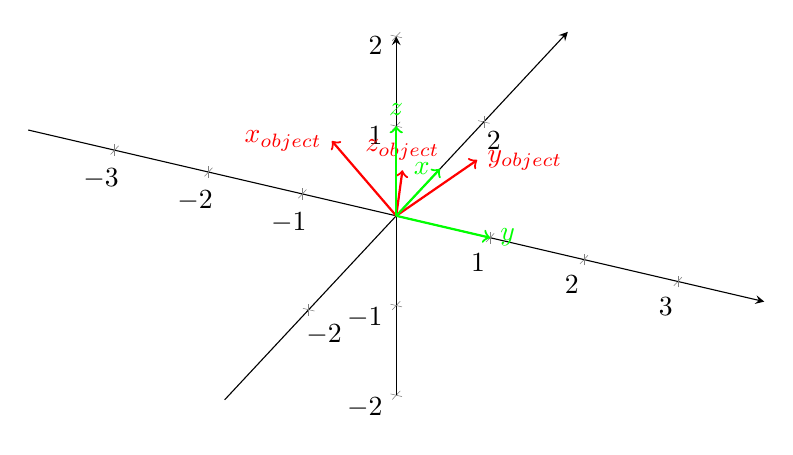
\begin{tikzpicture}
\begin{axis}[axis lines=middle, xmin=-2, xmax=2, ymin=-2,ymax=2, zmin=-2, zmax=2,axis equal,grid=both, scale=2]
\addplot3 [->, thick,  red] coordinates { (0,0,0) (.48,.82,.31)}node[right]{$y_{object}$};
\addplot3 [->, thick,  red] coordinates { (0,0,0) (-.83,.31,.47)}node[left]{$x_{object}$};
\addplot3 [->, thick,  red] coordinates { (0,0,0) (.29,-.48,.83)}node[above]{$z_{object}$};
\addplot3 [->, thick,  green] coordinates { (0,0,0) (1,0,0)}node[right]{$y$};
\addplot3 [->, thick,  green] coordinates { (0,0,0) (0,1,0)}node[left]{$x$};
\addplot3 [->, thick,  green] coordinates { (0,0,0) (0,0,1)}node[above]{$z$};
\end{axis}
\end{tikzpicture} \newpage

\section{3D frames}
3D frames are defined exactly like 2D frames, except the rotation matrices are used ${}^{A}_{B}R_{z'y'x'}(\alpha,\beta,\gamma)$. \\\\
\textbf{Example: }
Given frames: Frame \{A\} = universe,\\ 
Frame \{B\} = \{${}^{A}_{B}R_{z'y'x'}(45^\circ,10^\circ,10^\circ) ,{}^{A}P_{Borg}=\begin{bmatrix}
1 \\
1 \\
1
\end{bmatrix} $\},\\
Frame \{C\} = \{${}^{A}_{C}R_{z'y'x'}(90^\circ,130^\circ,-10^\circ) ,{}^{A}P_{Corg}=\begin{bmatrix}
-1  \\
-1  \\
-1
\end{bmatrix} $\},\\
Frame \{D\} = \{${}^{C}_{D}R_{z'y'x'}(45^\circ,45^\circ,45^\circ) ,{}^{C}P_{Dorg}=\begin{bmatrix}
1  \\
2  \\
3
\end{bmatrix} $\}\\\\
Given points: ${}^{A}P_{1}=\begin{bmatrix}
2  \\
-1 \\
1
\end{bmatrix}$, ${}^{B}P_{2}=\begin{bmatrix}
-2  \\
3\\
2
\end{bmatrix}$, ${}^{C}P_{3}=\begin{bmatrix}
1  \\
3 \\
-3
\end{bmatrix}$, ${}^{D}P_{4}=\begin{bmatrix}
-1  \\
1 \\
4
\end{bmatrix}$\\

\begin{tikzpicture}
\begin{axis}[axis lines=middle, xmin=-3, xmax=3, ymin=-3,ymax=3, zmin=-4, zmax=4,axis equal,grid=both, scale=2]
\addplot3 [->, thick,  blue] coordinates { (0,0,0) (2,-1,1)}node[above left]{$^AP_1$};

\addplot3 [->, thick,  black] coordinates { (1,1,1) (1.7,1.7,.83)}node[above left];
\addplot3 [->, thick,  black] coordinates { (1,1,1) (.32,1.72,1.17)}node[above left];
\addplot3 [->, thick,  black] coordinates { (1,1,1) (1.24,1,1.97)}node[above left];
\addplot3 [->, thick,  blue] coordinates { (1,1,1) (-1,4,3)}node[above left]{$^BP_2$};
\addplot3 [black] coordinates { (1,1,1) (1,1,1)}node[below]{$\{B\}$};

\addplot3 [->, thick,  black] coordinates { (-1,-1,-1) (-1,-1.64,-1.77)}node[above left];
\addplot3 [->, thick,  black] coordinates { (-1,-1,-1) (-1.98,-1.13,-.89)}node[above left];
\addplot3 [->, thick,  black] coordinates { (-1,-1,-1) (-1.17,-.25,-1.63)}node[above left];
\addplot3 [->, thick,  blue] coordinates { (-1,-1,-1) (0,2,-4)}node[above left]{$^CP_3$};
\addplot3 [black] coordinates { (-1,-1,-1) (-1,-1,-1)}node[above]{$\{C\}$};

\addplot3 [->, thick,  black] coordinates { (-3.49,.35,-3.44) (-3.86, -.57, -3.32)}node[above left];
\addplot3 [->, thick,  black] coordinates { (-3.49,.35,-3.44) (-4.42, .71, -3.55)}node[above left];
\addplot3 [->, thick,  black] coordinates { (-3.49,.35,-3.44) (-3.43, 0.20, -4.43)}node[above left];
\addplot3 [->, thick,  blue] coordinates { (-3.49,.35,-3.44) (-3.82, 1.03, -7.62)}node[above left]{$^DP_4$};
\addplot3 [black] coordinates { (-3.49,.35,-3.44) (-3.49,.35,-3.44) }node[above]{$\{D\}$};
\end{axis}
\end{tikzpicture}\\\\
Compute all transformation matrices: $^A_BT$, $^A_CT$, $^C_DT$, $^A_DT$, $^B_AT$, $^B_DT$\\\\
First lets compute $^A_BR_{z'y'x'}(45^\circ,10^\circ,10^\circ)= {}^A_BR_z {}^A_BR_y {}^A_BR_x=\\
\begin{bmatrix}
c45 & -s45 & 0\\
s45 & c45 & 0\\
0 & 0 & 1
\end{bmatrix}_z\begin{bmatrix}
c10 & 0 & s10\\
0 & 1 & 0\\
-s10 & 0 & c10
\end{bmatrix}_y
\begin{bmatrix}
1 & 0 & 0\\
0 & c10 & -s10\\
0 & s10 & c10
\end{bmatrix}_x=\\ \begin{bmatrix}
.71 & -.71 & 0\\
.71 & .71 & 0\\
0 & 0 & 1
\end{bmatrix}_z\begin{bmatrix}
.98 & 0 & .17\\
0 & 1 & 0\\
-.17 & 0 & .98
\end{bmatrix}_y
\begin{bmatrix}
1 & 0 & 0\\
0 & .98 & -.17\\
0 & .17 & .98
\end{bmatrix}_x=\begin{bmatrix}
.7 & -.68 &.24\\
.7 & .72 & -.001\\
-.17 & .17 & .97
\end{bmatrix}_{zyx}$\\
So we have $^A_BT=\begin{bmatrix}
 & ^A_BR_{z'y'x'}(45^\circ,10^\circ,10^\circ) & & ^AP_{Borg}\\
0 & 0 & 0 & 1 
\end{bmatrix}=\begin{bmatrix}
.7 & -.68 &.24 & 1\\
.7 & .72 & -.001 & 1\\
-.17 & .17 & .97 & 1\\
0 & 0 & 0 & 1
\end{bmatrix}$
\newpage
Similarly, $^A_CR_{z'y'x'}(90^\circ, 130^\circ,-10^\circ)=
\begin{bmatrix}
c90 & -s90 & 0\\
s90 & c90 & 0\\
0 & 0 & 1
\end{bmatrix}_z\begin{bmatrix}
c130 & 0 & s130\\
0 & 1 & 0\\
-s130 & 0 & c130
\end{bmatrix}_y
\begin{bmatrix}
1 & 0 & 0\\
0 & c-10 & -s-10\\
0 & s-10 & c-10
\end{bmatrix}_x=\begin{bmatrix}
0 &  -.98 & -.17\\
-.64 & -.13 & .75\\
-.77 & .11 & -.63
\end{bmatrix}$\\
^A_CT=\begin{bmatrix}
 & ^A_CR_{z'y'x'}(130^\circ,90^\circ,-10^\circ) & & ^AP_{Corg}\\
0 & 0 & 0 & 1 
\end{bmatrix}=\begin{bmatrix}
0 &  -.98 & -.17 & -1\\
-.64 & -.13 & .75 & -1\\
-.77 & .11 & -.63 & -1\\
0 & 0 & 0 & 1
\end{bmatrix}$\\\\
$^C_DR_{z'y'x'}(45^\circ, 45^\circ,45^\circ)=
\begin{bmatrix}
c45 & -s45 & 0\\
s45 & c45 & 0\\
0 & 0 & 1
\end{bmatrix}_z\begin{bmatrix}
c45 & 0 & s45\\
0 & 1 & 0\\
-s45 & 0 & c45
\end{bmatrix}_y
\begin{bmatrix}
1 & 0 & 0\\
0 & c45 & -s45\\
0 & s45 & c45
\end{bmatrix}_x=\begin{bmatrix}
0.5 & -0.15 & 0.85\\
0.5 & 0.85 & -0.15\\
-0.71 & 0.5 & 0.5      
\end{bmatrix}\\
$^C_DT=\begin{bmatrix}
 & ^C_DR_{z'y'x'}(45^\circ,45^\circ,45^\circ) & & ^CP_{Dorg}\\
0 & 0 & 0 & 1 
\end{bmatrix}=\begin{bmatrix}
0.5 & -0.15 & 0.85 & 1\\
0.5 & 0.85 & -0.15 & 2\\
-0.71 & 0.5 & 0.5 & 3\\
0 & 0 & 0 & 1
\end{bmatrix}$\\\\
$^A_DT = {}^A_CT {}^C_DT=\begin{bmatrix}
0 &  -.98 & -.17 & -1\\
-.64 & -.13 & .75 & -1\\
-.77 & .11 & -.63 & -1\\
0 & 0 & 0 & 1
\end{bmatrix}\begin{bmatrix}
0.5 & -0.15 & 0.85 & 1\\
0.5 & 0.85 & -0.15 & 2\\
-0.71 & 0.5 & 0.5 & 3\\
0 & 0 & 0 & 1
\end{bmatrix}=\begin{bmatrix}
-0.37 & -0.93 & 0.057 & -3.49\\
-0.92 & 0.36 & -0.15 & 0.35\\
0.12 & -0.11 & -0.99 & -3.44\\
0 & 0 & 0 & 1        
\end{bmatrix}$\\\\
\textbf{Computing the inverse of a transformation is also the same as it was in 2D but now we use a 4x4 homogeneous matrix}\\
$^B_AT={}^A_BT^{-1}=\begin{bmatrix}
 & ^A_BR_{z'y'x'}(45^\circ,10^\circ,10^\circ)^T & & -(^A_BR_{z'y'x'}(45^\circ,10^\circ,10^\circ)^T{}^AP_{Borg})\\
0 & 0 & 0 & 1 
\end{bmatrix}=\begin{bmatrix}
.7 & .7 & -.17 & -1.22\\
-.68 & .72 & .17 & -.21\\
.24 & -.001 & .97 & -1.21\\
0 & 0 & 0 & 1
\end{bmatrix}$\\\\
$^B_DT={}^B_AT{}^A_DT=\begin{bmatrix}
.7 & .7 & -.17 & -1.22\\
-.68 & .72 & .17 & -.21\\
.24 & -.001 & .97 & -1.21\\
0 & 0 & 0 & 1
\end{bmatrix}\begin{bmatrix}
-0.37 & -0.93 & 0.057 & -3.49\\
-0.92 & 0.36 & -0.15 & 0.35\\
0.12 & -0.11 & -0.99 & -3.44\\
0 & 0 & 0 & 1        
\end{bmatrix}=\begin{bmatrix}
-0.92 & -0.38 & 0.11 & -2.81\\
-0.39 & 0.86 & -0.32 & 1.81\\
0.028 & -0.33 & -0.94 & -5.40\\
 0 & 0 & 0 & 1        ]
\end{bmatrix}$
\newpage
\textbf{Compute} $^AP_2, ^AP_3, \text{ and } {}^AP_4$.\\\\
$^AP_2={}^A_BT{}^BP_2=\begin{bmatrix}
.7 & -.68 &.24 & 1\\
.7 & .72 & -.001 & 1\\
-.17 & .17 & .97 & 1\\
0 & 0 & 0 & 1
\end{bmatrix}\begin{bmatrix}
-2\\
3\\
2\\
1
\end{bmatrix}=\begin{bmatrix}
-1.93\\
1.76\\
3.8\\
1
\end{bmatrix}$\\\\
$^AP_3={}^A_CT{}^CP_3=\begin{bmatrix}
0 &  -.98 & -.17 & -1\\
-.64 & -.13 & .75 & -1\\
-.77 & .11 & -.63 & -1\\
0 & 0 & 0 & 1
\end{bmatrix}\begin{bmatrix}
1\\
3\\
-3\\
1
\end{bmatrix}=\begin{bmatrix}
-3.43\\
-4.31\\
.47\\
1
\end{bmatrix}$\\\\
$^AP_4={}^A_DT{}^DP_4=\begin{bmatrix}
-0.37 & -0.93 & 0.057 & -3.49\\
-0.92 & 0.36 & -0.15 & 0.35\\
0.12 & -0.11 & -0.99 & -3.44\\
0 & 0 & 0 & 1        
\end{bmatrix}\begin{bmatrix}
-1\\
1\\
4\\
1
\end{bmatrix}=\begin{bmatrix}
-3.82\\
1.03\\
-7.62\\
1
\end{bmatrix}$\\\\
\textbf{Compute} $^BP_1, ^BP_3, \text{ and } {} ^BP_4$.\\\\
$^BP_1={}^B_AT{}^AP_1=\begin{bmatrix}
.7 & .7 & -.17 & -1.22\\
-.68 & .72 & .17 & -.21\\
.24 & -.001 & .97 & -1.21\\
0 & 0 & 0 & 1
\end{bmatrix}\begin{bmatrix}
-1.93\\
1.76\\
3.8\\
1
\end{bmatrix}=\begin{bmatrix}
-.7\\
-2.11\\
.25\\
1
\end{bmatrix}$\\\\
$^BP_3={}^B_AT{}^AP_3=\begin{bmatrix}
.7 & .7 & -.17 & -1.22\\
-.68 & .72 & .17 & -.21\\
.24 & -.001 & .97 & -1.21\\
0 & 0 & 0 & 1
\end{bmatrix}\begin{bmatrix}
-3.43\\
-4.31\\
.47\\
1
\end{bmatrix}=\begin{bmatrix}
-6.69\\
-.91\\
.-1.58\\
1
\end{bmatrix}$\\\\
$^BP_4={}^B_DT{}^DP_4=\begin{bmatrix}
-0.92 & -0.38 & 0.11 & -2.81\\
-0.39 & 0.86 & -0.32 & 1.81\\
0.028 & -0.33 & -0.94 & -5.40\\
 0 & 0 & 0 & 1        ]
\end{bmatrix}\begin{bmatrix}
-1\\
1\\
4\\
1
\end{bmatrix}=\begin{bmatrix}
-1.83\\
1.78\\
-9.52\\
1
\end{bmatrix}$\\\\
\textbf{Compute} $^CP_1, ^CP_2, \text{ and } {} ^CP_4$.\\\\
$^CP_1={}^C_AT{}^AP_1=\begin{bmatrix}
0 & -.64 & -.77 & -1.41\\
-.98 & -.13 & .11 & -1.01\\
-.17 & .75 & -.63 & -.05\\
0 & 0 & 0 & 1
\end{bmatrix}\begin{bmatrix}
2\\
-1\\
1\\
1
\end{bmatrix}=\begin{bmatrix}
-1.53\\
-2.73\\
-1.79\\
1
\end{bmatrix}$\\\\
$^CP_2={}^C_AT{}^AP_2=\begin{bmatrix}
0 & -.64 & -.77 & -1.41\\
-.98 & -.13 & .11 & -1.01\\
-.17 & .75 & -.63 & -.05\\
0 & 0 & 0 & 1
\end{bmatrix}\begin{bmatrix}
-1.93\\
1.76\\
3.8\\
1
\end{bmatrix}=\begin{bmatrix}
-5.45\\
1.08\\
-.79\\
1
\end{bmatrix}$\\\\
$^CP_4={}^C_DT{}^DP_4=\begin{bmatrix}
0.5 & -0.15 & 0.85 & 1\\
0.5 & 0.85 & -0.15 & 2\\
-0.71 & 0.5 & 0.5 & 3\\
0 & 0 & 0 & 1
\end{bmatrix}\begin{bmatrix}
-1\\
1\\
4\\
1
\end{bmatrix}=\begin{bmatrix}
3.77\\
1.77\\
6.21\\
1
\end{bmatrix}$\\\\
\textbf{Compute} $^DP_1, ^DP_2, \text{ and } {}^DP_3$.\\\\
$^DP_1={}^D_AT{}^AP_1=\begin{bmatrix}
-.37 & -.92 & .12 & -.55\\
-.93 & .36 & -.11 & -3.74\\
.06 & -.15 & -.99 & -3.14\\
0  &  0  &  0  &  1  
\end{bmatrix}\begin{bmatrix}
2\\
-1\\
1\\
1
\end{bmatrix}=\begin{bmatrix}
-.25\\
-6.06\\
-3.86\\
1
\end{bmatrix}$\\\\
$^DP_2={}^D_AT{}^AP_2=\begin{bmatrix}
-.37 & -.92 & .12 & -.55\\
-.93 & .36 & -.11 & -3.74\\
.06 & -.15 & -.99 & -3.14\\
0  &  0  &  0  &  1  
\end{bmatrix}\begin{bmatrix}
-1.93\\
1.76\\
3.8\\
1
\end{bmatrix}=\begin{bmatrix}
-1\\
-1.73\\
-7.27\\
1
\end{bmatrix}$\\\\
$^DP_3={}^D_AT{}^AP_3=\begin{bmatrix}
-.37 & -.92 & .12 & -.55\\
-.93 & .36 & -.11 & -3.74\\
.06 & -.15 & -.99 & -3.14\\
0  &  0  &  0  &  1  
\end{bmatrix}\begin{bmatrix}
-3.43\\
-4.31\\
.47\\
1
\end{bmatrix}=\begin{bmatrix}
4.75\\
-2.15\\
-3.15\\
1
\end{bmatrix}$\\\\
\section{How to find euler angles from rotation matrix}
Notation:$c\theta = cos(\theta)$ and $s\theta=sin(theta)$\\\\
${}^{A}_{B}R_{z'y'x'}(\alpha,\beta,\gamma)={}^{A}_{B}R_{z'}(\alpha){}^{A}_{B}R_{y'}(\beta){}^{A}_{B}R_{x'}(\gamma) = 
\begin{bmatrix}
c\alpha & -s\alpha & 0\\
s\alpha & c\alpha & 0 \\
0 & 0 & 1
\end{bmatrix}
\begin{bmatrix}
c\beta & 0 & s\beta\\
0 & 1 & 0 \\
-s\beta & 0 & c\beta
\end{bmatrix}
\begin{bmatrix}
1 & 0 & 0\\
0 & c\gamma & -s\gamma \\
0 & s\gamma & c\gamma
\end{bmatrix} =
\begin{bmatrix}
c\alpha c\beta & s\gamma s\beta c\alpha - c\gamma s\alpha & c\gamma s\beta c\alpha + s\gamma s\alpha\\
s\alpha c\beta & s\gamma s\beta s\alpha + c\gamma c\alpha & c\gamma s\beta s\alpha - s\gamma c\alpha \\
-s\beta & s\gamma c\beta & c\gamma c\beta
\end{bmatrix}=
\begin{bmatrix}
r_{11} & r_{12} & r_{13}\\
r_{21} & r_{22} & r_{23} \\
r_{31} & r_{32} & r_{33}
\end{bmatrix}$
\\\\
$\beta_1 = -arcsin(r31)\\
\beta_2 = 180^{\circ}-\beta_1\\\\
\alpha_1 = arctan(\frac{r_{21}}{r_{11}}) (\text{if } \frac{r_{11}}{c\beta_1} < 0 \text{ and } -90^{\circ} < \alpha_1 < 90^{\circ}, \text{ add } 180^{\circ})\\\\
\alpha_2 = arctan(\frac{r_{21}}{r_{11}}) (\text{if } \frac{r_{11}}{c\beta_2} < 0 \text{ and } -90^{\circ} < \alpha_2 < 90^{\circ}, \text{ add } 180^{\circ})\\\\
\gamma_1 = arctan(\frac{r_{32}}{r_{33}}) (\text{if } \frac{r_{33}}{c\beta_1} < 0 \text{ and } -90^{\circ} < \gamma_1 < 90^{\circ}, \text{ add } 180^{\circ})\\\\
\gamma_2 = arctan(\frac{r_{32}}{r_{33}}) (\text{if } \frac{r_{33}}{c\beta_2} < 0 \text{ and } -90^{\circ} < \gamma_2 < 90^{\circ}, \text{ add } 180^{\circ})\\\\$
Notes: If $\beta = 90^{\circ}$ then the angles are not solvable for. This is the infamous situation of gimbal lock where two of the rotational axes line up creating the case of a singular rotation matrix.\\
video: \url{https://www.youtube.com/watch?v=zc8b2Jo7mno}\\\\
2. The "$\frac{r_{11}}{c\beta_1} < 0 \text{ and } -90^{\circ} < \alpha_1 < 90^{\circ}, \text{ add } 180^{\circ})$" is used to resolve the ambiguity of the arctan function. The ambiguity stems from $tan(\theta)=tan(\theta+180)=a$ so is $arctan(a)=\theta$ or $arctan(a)=\theta+180$? In our case, We know that $cos(\alpha)=\frac{r_{11}}{cos(\beta)}$, by analyzing the sign from this equation we can determine what quadrant $\alpha$ will lie in, resolving the inherent ambiguity. This is what the atan2 function in programming languages was built to do.

\section{Solving euler angles example}
Given frames: Frame \{A\} = universe,\\ 
Frame \{B\} = \{${}^{A}_{B}R=\begin{bmatrix}
-.18 & .24 & .96\\
-.18 & .95 & -.27\\
-.97 & -.23 & -.13
\end{bmatrix} ,{}^{A}P_{Borg}=\begin{bmatrix}
-1  \\
4  \\
3
\end{bmatrix} \}$\\
Given points: ${}^{A}P_{1}=\begin{bmatrix}
2  \\
3 \\
2
\end{bmatrix}$, ${}^{B}P_{2}=\begin{bmatrix}
-1  \\
-2 \\
2
\end{bmatrix}$\\\\
\textbf{1.)} Find ${}^{B}P_{1}$ and ${}^{A}P_{2}$\\\\
${}^{A}_{B}T=\begin{bmatrix}
-.18 & .24 & .96 & -1\\
-.18 & .95 & -.27 & 4\\
-.97 & -.23 & -.13 &  3\\
0 & 0 & 0 & 1
\end{bmatrix}$\\
${}^{B}_{A}T={}^{A}_{B}T^{-1}=\begin{bmatrix}
{}^{A}_{B}R^T & -({}^{A}_{B}R^T{}^{A}P_{Borg})\\
0 & 0 & 0 & 1
\end{bmatrix}=
\begin{bmatrix}
-.18 & -.18 & -.97 & -3.45\\
.24 & .95 & -.23 & 2.87\\
.96 & -.27 & -.13 & -2.43\\
0 & 0 & 0 & 1
\end{bmatrix}$\\\\
${}^{B}P_{1}={}^{B}_{A}T{}^{A}P_{1}=\begin{bmatrix}
-.18 & -.18 & -.97 & -3.45\\
.24 & .95 & -.23 & 2.87\\
.96 & -.27 & -.13 & -2.43\\
0 & 0 & 0 & 1
\end{bmatrix}
\begin{bmatrix}
2\\
3\\
2\\
1
\end{bmatrix}=
\begin{bmatrix}
-6.29\\
5.74\\
-1.58\\
1
\end{bmatrix}$\\\\
${}^{A}P_{2}={}^{A}_{B}T{}^{B}P_{2}=\begin{bmatrix}
-.18 & .24 & .96 & -1\\
-.18 & .95 & -.27 & 4\\
-.97 & -.23 & -.13 &  3\\
0 & 0 & 0 & 1
\end{bmatrix}
\begin{bmatrix}
-1\\
-2\\
2\\
1
\end{bmatrix}=
\begin{bmatrix}
.62\\
1.72\\
4.17\\
1
\end{bmatrix}$\\\\\\
\textbf{2.) (Use calculator in degree mode!)}\\
$\beta_1=-arcsin(r_{31})=-arcsin(-.97)=75^{\circ}$\\
$\beta_2=180^{\circ}-\beta_1=180^{\circ}-75^{\circ}=105^{\circ}$\\
$\alpha_1=arctan(\frac{r_{21}}{r_{11}})=arctan(\frac{-.18}{-.18})=45^{\circ}$\\
$\text{since }\frac{r_{11}}{cos(\beta_1)}=\frac{-.18}{.26} < 0 \text{ and } -90^{\circ} < 45^{\circ} < 90^{\circ},
\text{ we add } 180^{\circ} \text{ to } \alpha_1, \alpha_1=225^{\circ}$
$\alpha_2=arctan(\frac{r_{21}}{r_{11}})=arctan(\frac{-.18}{-.18})=45^{\circ}, \frac{r_{11}}{cos(\beta_2)}=\frac{-.18}{-.26} > 0$(so no need to add anything)\\
$\gamma_1=arctan(\frac{r_{32}}{r_{33}})=arctan(\frac{-.23}{-.13})=60^{\circ}$\\
$\text{since }\frac{r_{33}}{cos(\beta_1)}=\frac{-.13}{.26} < 0 \text{ and } -90^{\circ} < 60^{\circ} < 90^{\circ},
\text{ we add } 180^{\circ} \text{ to } \gamma_1, \gamma_1=240^{\circ}$
$\gamma_2=arctan(\frac{r_{32}}{r_{33}})=arctan(\frac{-.23}{-.13})=45^{\circ}, \frac{r_{33}}{cos(\beta_2)}=\frac{-.13}{-.26} > 0$(so no need to add anything)\\\\
You will always have two sets of possible answers.\\
Set 1: $(\alpha_1, \beta_1, \gamma_1)=(225^{\circ}, 75^{\circ}, 240^{\circ})$\\
Set 2: $(\alpha_1, \beta_1, \gamma_1)=(45^{\circ}, 105^{\circ},60 ^{\circ})$\\\\
To verify, make sure:\\
${}^{A}_{B}R=\begin{bmatrix}
-.18 & .24 & .96 \\
-.18 & .95 & -.27 \\
-.97 & -.23 & -.13 \\
\end{bmatrix}=
\begin{bmatrix}
c\alpha_1 & -s\alpha_1 & 0\\
s\alpha_1 & c\alpha_1 & 0 \\
0 & 0 & 1
\end{bmatrix}
\begin{bmatrix}
c\beta_1 & 0 & s\beta_1\\
0 & 1 & 0 \\
-s\beta_1 & 0 & c\beta_1
\end{bmatrix}
\begin{bmatrix}
1 & 0 & 0\\
0 & c\gamma_1 & -s\gamma_1 \\
0 & s\gamma_1 & c\gamma_1
\end{bmatrix}=
\begin{bmatrix}
c\alpha_2 & -s\alpha_2 & 0\\
s\alpha_2 & c\alpha_2 & 0 \\
0 & 0 & 1
\end{bmatrix}
\begin{bmatrix}
c\beta_2 & 0 & s\beta_2\\
0 & 1 & 0 \\
-s\beta_2 & 0 & c\beta_2
\end{bmatrix}
\begin{bmatrix}
1 & 0 & 0\\
0 & c\gamma_2 & -s\gamma_2 \\
0 & s\gamma_2 & c\gamma_2
\end{bmatrix}$

\section{rotate and translate a point}
So far we have solved the problem of taking a point in some frame and interpreting that same point in another frame. This section will address the problem of - given a frame, and a point in that frame, how do we translate and rotate the point? Fortunately for us, it is similar to what we have done so far. \\
Lets say we are given:\\
Frame \{A\} = universe,\\ 
Frame \{B\} = \{${}^{A}_{B}R=\begin{bmatrix}
-.18 & .24 & .96\\
-.18 & .95 & -.27\\
-.97 & -.23 & -.13
\end{bmatrix} ,{}^{A}P_{Borg}=\begin{bmatrix}
-1  \\
4  \\
3
\end{bmatrix}\}\\
{}^{A}P_{1}=\begin{bmatrix}
1  \\
2  \\
0
\end{bmatrix}, {}^{B}P_{2}=\begin{bmatrix}
0  \\
1  \\
1
\end{bmatrix}$\\
Rotate and translate ${}^{A}P_{1}$ and ${}^{B}P_{2}$ by $R_{z'y'x'}(90^{\circ},0,0)$ and translate by vector $\begin{bmatrix}
1  \\
2  \\
3
\end{bmatrix}$\\\\
We can construct the transformation just like we did for frames(sinces its essentially the same thing, ${}^{A}_{B}R^T$, tells us how to move A to turn it into B). T will tells us how to move our point within a frame.\\\\
$T = \begin{bmatrix}
0 & -1 & 0 & 1\\
1 & 0 & 0 & 2\\
0 & 0 & 1 &  3\\
0 & 0 & 0 & 1
\end{bmatrix}$\\\\
${}^{A}P_{1r}= T{}^{A}P_{1}=\begin{bmatrix}
0 & -1 & 0 & 1\\
1 & 0 & 0 & 2\\
0 & 0 & 1 &  3\\
0 & 0 & 0 & 1
\end{bmatrix}\begin{bmatrix}
1  \\
2  \\
0  \\
1
\end{bmatrix}=\begin{bmatrix}
-1  \\
3  \\
3  \\
1
\end{bmatrix}$\\\\
${}^{B}P_{2r}= T{}^{B}P_{2}=\begin{bmatrix}
0 & -1 & 0 & 1\\
1 & 0 & 0 & 2\\
0 & 0 & 1 &  3\\
0 & 0 & 0 & 1
\end{bmatrix}\begin{bmatrix}
0  \\
1  \\
1  \\
1
\end{bmatrix}=\begin{bmatrix}
0  \\
2  \\
4  \\
1
\end{bmatrix}$\\
\begin{tikzpicture}
\begin{axis}[axis lines=middle, xmin=-5, xmax=5, ymin=-5,ymax=5, zmin=-5, zmax=5,axis equal,grid=both, scale=2]
\addplot3[->, thick,  green] coordinates { (0,0,0) (2,2,0)}node[above left]{$\mathbf{{}^{A}P_1}$};
\addplot3[->, thick,  red] coordinates { (0,0,0) (-1,3,3)}node[above left]{$\mathbf{{}^{A}P_{1r}}$};

\addplot3 [->, thick,  black] coordinates { (-1,4,3) (-1.12,3.88,2.02)}node[above left];
\addplot3 [->, thick,  black] coordinates { (-1,4,3) (-.75,4.96,2.85)}node[above left];
\addplot3 [->, thick,  black] coordinates { (-1,4,3) (-.04,3.74,2.91)}node[above left];
\addplot3 [black] coordinates { (-1,4,3) (-1,4,3)}node[above]{$\{B\}$};
\addplot3[->, thick,  green] coordinates { (-1,4,3) (.21,4.69,2.76)}node[above left]{$\mathbf{{}^{B}P_2}$};
\addplot3[->, thick,  red] coordinates { (-1,4,3) (3.84,4.86,2.35)}node[above left]{$\mathbf{{}^{B}P_{2r}}$};
\end{axis}
\end{tikzpicture}

We can also use the inverse of T, to undo the transformation.\\
$T^{-1}=\begin{bmatrix}
R^T & -(R^Tt_{vec})\\
0 & 0 & 0 & 1
\end{bmatrix}$\\\\
${}^{A}P_{1}= T^{-1}{}^{A}P_{1r}=\begin{bmatrix}
0 & 1 & 0 & 2\\
-1 & 0 & 0 & -1\\
0 & 0 & 1 &  3\\
0 & 0 & 0 & 1
\end{bmatrix}\begin{bmatrix}
-1  \\
3  \\
3  \\
1
\end{bmatrix}=\begin{bmatrix}
1  \\
2  \\
0  \\
1
\end{bmatrix}$\\\\
${}^{B}P_{2}= T^{-1}{}^{B}P_{2r}=\begin{bmatrix}
0 & 1 & 0 & 2\\
-1 & 0 & 0 & -1\\
0 & 0 & 1 &  3\\
0 & 0 & 0 & 1
\end{bmatrix}\begin{bmatrix}
0  \\
2  \\
4  \\
1
\end{bmatrix}=\begin{bmatrix}
0  \\
1  \\
1  \\
1
\end{bmatrix}$\\\\

\subsection{Solving for angles between vectors}
For every pair of a vectors there exist an angle between them, on some rotational axis(not x,y or z. More on this in next section). To find this angle we use the dot product formula:\\\\
$arccos(\frac{v_1 \cdot v_2}{|v_1||v_2|})=\theta$ where $\theta$ is the angle between vectors $v_1$ and $v_2$.\\\\
\textbf{Example:}\\
Find angle between $^BP_2$ and $^BP_{2r}$ from previous question.\\
$\theta=arccos(\frac{^BP_2 \cdot {}^BP_{2r}}{|{}^BP_2||{}^BP_{2r}|})=28.13^\circ$ 

\section{Angle-axis form}
Angle-axis form parameterizes a 3D rotation with one axis(vector in 3D(red in image)), and one angle of rotation on plane perpendicular to axis(green below).\\\\
\tdplotsetmaincoords{70}{110}
\begin{tikzpicture}[scale=3,tdplot_main_coords]
    \filldraw[
        draw=green,%
        fill=green!20,%
    ]          (-1,-1,-.5)
            -- (-1,1,.5)
            -- (1,1,.5)
            -- (1,-1,-.5)
            -- cycle;
    \draw[thick,->] (0,0,0) -- (1,0,0) node[anchor=north east]{$x$};
    \draw[thick,->] (0,0,0) -- (0,1,0) node[anchor=north west]{$y$};
    \draw[thick,->] (0,0,0) -- (0,0,1) node[anchor=south]{$z$};
    \draw[thin,->,red] (0,0,0) -- (0,-.5,1) node[left] {$n$};
\end{tikzpicture}\\\\
Rodrigues formula: $v_r=( v )cos(\theta) + (n \times v)sin(\theta) + (n)(n \cdot v)(1-cos(\theta))$\\
\textbf{Note: } rodrigues formula is used for rotating a vector $v$, make sure $n$ is unit normal vector.\\\\
\textbf{Example: } Rotate vector $v=\begin{bmatrix}
1\\
-2\\
1
\end{bmatrix}$ by $75^\circ$ along axis $n=\begin{bmatrix}
1\\
2\\
3
\end{bmatrix}
$. \\\\
First we must consider the unit vector version of $n$, we can get this vector by dividing $n$ by the magnitude of $n$($|n|$).\newpage
$|n|=\sqrt{1^2+2^2+3^2}=\sqrt{14} \approx 3.74$\\
$\hat{n}=\frac{n}{|n|}=\frac{\begin{bmatrix}
1\\
2\\
3
\end{bmatrix}}{\sqrt{14}}=\begin{bmatrix}
\frac{1}{\sqrt{14}}\\
\frac{2}{\sqrt{14}}\\
\frac{3}{\sqrt{14}}
\end{bmatrix}$\\
$\hat{n} \times v = \begin{bmatrix}
\frac{1}{\sqrt{14}}\\
\frac{2}{\sqrt{14}}\\
\frac{3}{\sqrt{14}}
\end{bmatrix} \times
\begin{bmatrix}
 1\\
 -2\\
 1
\end{bmatrix}=\begin{bmatrix}
2\\
1\\
-1
\end{bmatrix}$\\\\
$\hat{n} \cdot v = 
\begin{bmatrix}
\frac{1}{\sqrt{14}}\\
\frac{2}{\sqrt{14}}\\
\frac{3}{\sqrt{14}}
\end{bmatrix} \cdot
\begin{bmatrix}
 1\\
 -2\\
 1
\end{bmatrix}  
=0$\\\\
$v_r=( v )cos(\theta) + (\hat{n} \times v)sin(\theta) + (\hat{n})(\hat{n} \cdot v)(1-cos(\theta))=\begin{bmatrix}
1\\
-2\\
1
\end{bmatrix}cos(75^\circ)+ \begin{bmatrix}
2\\
1\\
-1
\end{bmatrix}sin(75^\circ) + \begin{bmatrix}
0\\
0\\
0
\end{bmatrix}(1-cos(75^\circ))=\begin{bmatrix}
2.32\\
0\\
-.77
\end{bmatrix}$\\\\
\tdplotsetmaincoords{70}{110}
\begin{tikzpicture}[scale=3,tdplot_main_coords]
    \filldraw[
        draw=green,%
        fill=green!20,%
    ]          (-1,-1,1)
            -- (-1,1,-.33)
            -- (1,1,-1)
            -- (1,-1,.33)
            -- cycle;
    \draw[thick,->] (0,0,0) -- (1,0,0) node[anchor=north east]{$x$};
    \draw[thick,->] (0,0,0) -- (0,1,0) node[anchor=north west]{$y$};
    \draw[thick,->] (0,0,0) -- (0,0,1) node[anchor=south]{$z$};
    \draw[thin,->,red] (0,0,0) -- (.27,.53,.8) node[left] {$n$};
    \draw[thin,->,blue] (0,0,0) -- (1,-2,1) node[left] {$v$};
    \draw[thin,->,blue] (0,0,0) -- (2.32,0,-.77) node[left] {$v_r$};
\end{tikzpicture}
\end{document}
